\section{Proposed work}

Here, I explain the system to be implemented and the experiments to be conducted.

\subsection{Potentiation in an NK landscape}

%Earlier work looking at potentiation provides evidence that potentiating mutations can be highly epistatic [CITE?]. 
%Even though we are using a simple bitstring genotype, we need an environment that allows for epistatic interactions between the bits. 
Since I expect that epistatic interactions play a key role in potentiating mutations, the simple bitstring model must contain some level of epistasis. 
Fortunately, this is an inherent property of NK landscapes \citep{kauffmanGeneralTheoryAdaptive1987}, where $N$ is the length of the bitstring and $K$ is the number of additional bits that epistatically interact to determine the fitness of each position in the bitstring. 
As such, not only are NK landscapes epistatic, but the degree of epistasis is a parameter I can vary, allowing for clean comparisons of dynamics at different levels of epistasis. 

Quantifying potentiation requires a target trait, as we must designate whether lineages are ``successful''. 
All genotypes in the NK landscape, as I consider it, map to a scalar value. 
I will construct the landscapes such that, for each bit position, each unique combination of $K + 1$ bits grants a score between 0 and 1 that is random but set for the duration of the landscape. 
The total score of a genotype is then the sum of scores for all positions in the bitstring. 
Since I use floating-point numbers, the randomness of the bit position scores allows me to assume that a unique global optimum exists in each landscape. 
I therefore define the successful trait as having exactly this optimal bitstring. 
Conveniently, the distance to the target trait is just the Hamming distance between the optimal bitstring and the genotype in question. 

% \begin{figure}[h!]
%     \centering
%     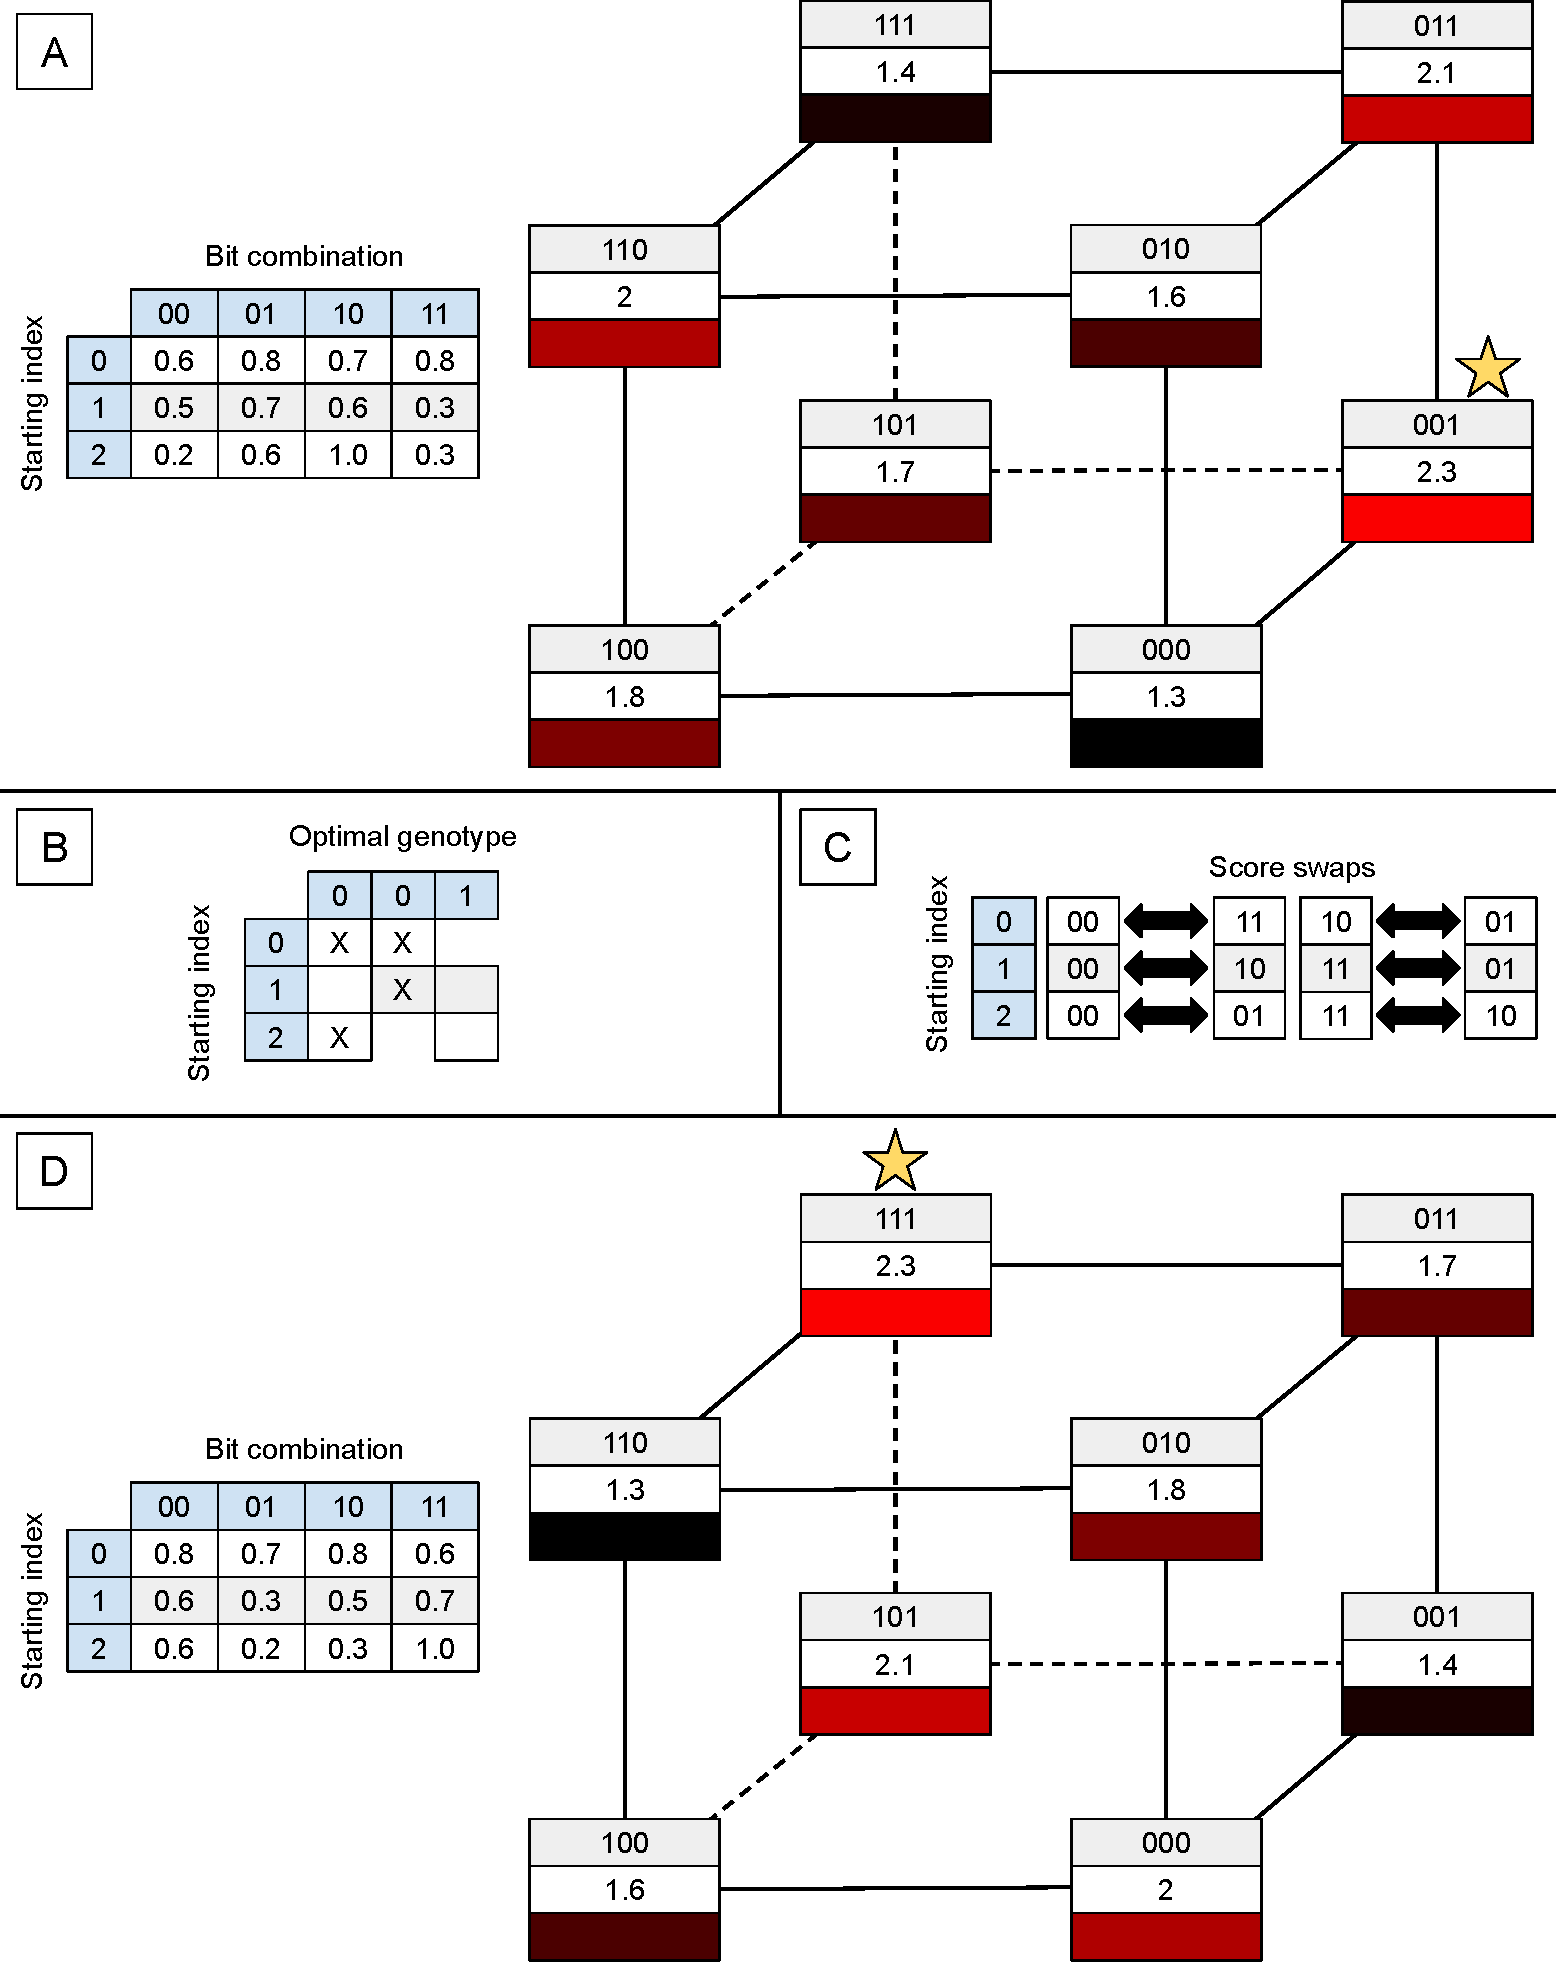
\includegraphics[width=0.9\textwidth]{04_simplified_model/media/rotating_landscape.pdf}
%     \caption{
%         An example of rotating an NK landscape where $N=3$ and $K=1$. 
%         Panel A shows the original landscape, including the score table and the visualized landscape. 
%         The yellow star shows the genotype with optimal fitness, 001. 
%         Panel B shows the mask of which bits need flipped, in this case the first two. 
%         These flips are demonstrated in Panel C.
%         At the first starting index both bits are flipped, while only one bit is flipped in the other indices. 
%         Finally, Panel D shows the resulting score table and landscape, which is isomorphic to the first but now 111 has maximal fitness.
%     }
%     \label{fig:simplified_model:rotating_landscape}
% \end{figure}

% We make one change to the NK landscape to make our analysis easier. 
% Traditionally in bitstring models, the distance between two bitstrings is calculated as their Hamming distance.
% To make comparisons with the global optimum easier, we propose to ``rotate'' the NK landscape. 
% Once the global optimum is known (in this case, found via brute force enumeration), the scoring rules of the landscape can be changed such that the global optimum occurs at the bitstring of all ones. 
% To accomplish this, for every zero in the original global optimal bitstring, we must swap the scores anywhere this bit is used. 
% This does not change the topology of the landscape, it merely re-labels the genotypes within.
% Figure \ref{fig:simplified_model:rotating_landscape} shows an example 
% Note that this is equivalent to XOR-ing a bitstring with the complement of the global optimum bitstring before evaluating its score.
% Once this transformation is complete, the distance to the optimal, successful, genotype is simply the number of zeros in a genome. 

I will conduct evolution like a traditional synchronous-generation genetic algorithm. 
I will seed the initial population of bitstrings with the genotype being tested, and evaluate each bitstring on the landscape. 
After this evaluation, I will select parents via a mix of elite selection (to ensure the optimal genotype persists if it is discovered) and tournament selection. 
Finally, all parents will be copied and possibly mutated, creating the next generation to be evaluated. 
I will then repeat this process until a stopping criterion is met. 

Quantifying the potentiation of a genotype is done by seeding some number of evolutionary replicates with that genotype and measuring the percentage of those replicates that evolve the target trait (as originally introduced in \citet{blountHistoricalContingencyEvolution2008}). %the percentage of replicates that evolve the target behavior when starting at that genotype. 
Typically, this is only measurable via multiple replay experiments that restart evolution at specific points along a lineage. 
Because I am using bitstrings, I am able to enumerate potentiation for \textit{all} possible genotypes in a landscape, creating a ``potentiation landscape''. 
This requires nontrivial effort, as there are $2^{N}$ possible genotypes in an $N$-length bitstring, and analyzing each genotype requires multiple evolutionary replicates started from it (here I use 50). 
%Once the 50 replicates for a given genotype are finished, I calculate potentiation as the percentage of those replicates evolved the target trait. 
%For the first time, we will be able to observe how potentiation changes with every step, both along a lineage and in the neighboring steps that could have been taken. 
This approach limits the size of landscapes that I can enumerate. 
As such, I propose to start by analyzing landscapes where $N \in \{10,12,14,16\}$ bits.
For each of these $N$ values, I will also vary $K \in [0, N - 1]$.
To ensure we observe the diversity landscapes can have at a particular combination of $N$ and $K$, I will enumerate the potentiation landscape for 30 landscapes at each pair of values. 

% First, we define the patterns of potentiation that we hope to observe in the system. 
% These are refined from the exploratory work of Chapter \ref{chap:replaying_associative_learning}, and are subject to change as we finish Chapters \ref{chap:replaying_associative_learning} and \ref{chap:varying_environments}.
% The three types of potentiation are: 
% \begin{enumerate}
%     \item Mutating toward the behavior, reducing the number of mutations to get there in the future
%     \item Shifting toward another genotype with the behavior that has a larger fitness advantage
%     \item Moving to another point in the genotype space such that the path toward the behavior becomes easier to traverse
% \end{enumerate}
% The three types of potentiation are visualized in Figure \ref{fig:06:conceptual_figure}

% We have constructed a bitstring model that allows for all three types of potentiation. 


% \begin{figure}
%     \centering
%     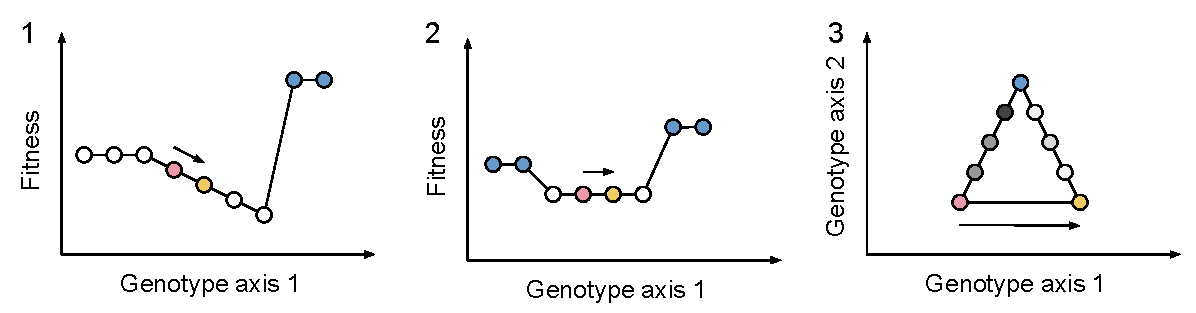
\includegraphics[width=0.9\textwidth]{04_simplified_model/media/potentiation_types_conceptual_figure.pdf}
%     \caption{
%     A conceptual figure demonstrating the three types of potentiating mutations.
%     The first two subplots show fitness on the y-axis, while the final subplot requires two genotype-space axes. 
%     All plots show the starting genotype in red, the potentiated mutant in yellow, and one or more genotypes with the focal trait in blue.
%     Arrows also show the mutation. 
%     The final subplot shows fitness of intermediate points on a grayscale axis with lighter colors being more fit.}
%     \label{fig:06:conceptual_figure}
% \end{figure}

\subsection{Proposed comparative analyses}

I plan to conduct two comparisons of potentiation: one between the NK landscape and the associative learning Avida domain, and the other across different $N$ and $K$ values within the NK landscape. 
However, the measurements taken in the associative learning domain were looking at potentiation along a lineage, not over the entire landscape (see \ref{sub:potentiation_measures} for the list of measurements). 
I will calculate the lineage metrics in the NK landscape by rerunning replicates at particular genotypes, tracking the evolving phylogenies. 
Specifically, I will target genotypes with low potentiation values, below 10\%, in order to create a fair comparison with the low initial potentiation seen in the associative learning results. 
Here, however, we do not need to perform replay replicates along these lineages, as we already know the potentiation of every possible genotype.
We merely need to map genotypes along the lineage with their potentiation values. 
Once potentiation has been assigned to every genotype along the lineage, we can calculate the potentiation measurements as normal. 

After these measurements have been collected, I will compare the distributions of each with those found in the associative learning environment of Chapter \ref{chap:replaying_associative_learning}.
As an example, I will test if there is a significant difference in the largest single-step potentiation gain between the two systems. 
Not all measurements translate to this system, but largest single-step potentiation gain/loss, the distance to the target trait from the potentiating mutations, and distributions of fitness effect apply equally to both systems. 
This will provide the first comparison of potentiation across environments and representations. 
If the distributions are similar, that would be strong evidence that there are general trends in potentiation. 
If, instead, significant differences exist, that will also provide information on what our simplified model might be missing. 

Next, I plan to perform a similar analysis across $K$ values in the NK landscape. 
Since $K$ controls the level of epistasis in the landscape, these tests will highlight the effect that epistasis has on our potentiation measurements. 
I will perform this analysis for each of the $N$ values tested. 
I will compare the relevant potentiation measurements across the set of $K$ values, seeing which ones statistically differ. 
%For example, does the fitness effect of potentiating mutations change as we increase the level of epistasis in the system? 
For example, I expect increased epistasis to make the landscapes more deceptive and thus increase the effect size of potentiating mutations.
Likewise, I will examine the consistency of the effect of $K$ on potentiation, by comparing fixed $K$ values across each $N$.

For both of these comparisons, I will conduct a Kruskal-Wallis test across all groups to see if any significant difference is found \citep{kruskal_use_1952}. 
If a difference is present, I will then conduct pairwise Mann-Whitney-Wilcoxon tests to determine which pairs of groups differ \citep{10.2307/3001968}.
Finally, I will apply Holm-Bonferroni corrections for multiple comparisons where needed \citep{holmSimpleSequentiallyRejective1979}.

% I propose a set of analyses that expand upon the work proposed in Chapter \ref{chap:replaying_associative_learning}. 
% Overall, I will enumerate multiple landscapes for various values of $N$ and $K$, calculating potentiation for every possible genotype. 
% This will allow us to compare the fitness landscape with the ``potentiation landscape'' for the first time. 
% As such, we can examine the relationships between fitness, potentiation, the distance to the target genotype, $N$, and $K$.
% Additionally, in enumerating genotype space, we will be running multiple evolutionary replicates from each genotype. 
% We can examine the dominant lineage of any of these replicates, allowing us to see how potentiation changed over time. 
% This allows us to compare potentiation in this system to that of Chapter \ref{chap:replaying_associative_learning}, which looked at the potentiation of associative learning in Avida. 

% To map the potentiation landscape, I will quantify potentiation at every possible genotype. 
% In our bitstring model, that can be accomplished by testing every bitstring in $[0, 2^{N} - 1]$.
% For a given genotype, we measure potentiation in the same way as previous work \citep{blountHistoricalContingencyEvolution2008} (Chapter \ref{chap:alife_submission}); we run a large number of evolutionary replicates starting from that genotype and calculate the percetange of those replicates that evolve the target trait. 
% This has traditionally been done along a lineage, but the same test holds for arbitrary genotypes. 
% The one difference is the time allowed in those evolutionary replicates. 
% Along a lineage, time is typically controlled such that the number of generations before that time point is subtracted from a total generation budget, ensuring that genotypes later in the lineage see fewer generations than those earlier. 
% Here we simply give all genotypes the same budget of 5,000 generations, which should be more than enough to traverse stable point. 
% I will perform these enumerations on 50 landscapes per treatment, varying $N \in [10,16]$ and $K \in [0,4]$ for a total of 35 treatments and 1750 landscapes. 
% This requires substantial computation effort, but preliminary experiments show that a 10-bit landscape can be fully enumerated in a matter of hours (a comparable amount of time to one initial replicate in Chapter \ref{chap:alife_submission}).

% Once the landscapes have been enumerated, I will analyze the relationships within and between treatments. 
% Within a treatment (a combination of $N$ and $K$), I will examine the distributions of potentiation of all genotypes.
% A Kruskal-Wallis test will determine if any significant variation exists among these distributions \citep{kruskal_use_1952}. 
% In each treatment, I will also inspect the relationship between fitness and potentiation for a sampling of landscapes. 
% I hypothesize that low potentiation can arise from populations reaching a local optima, preventing them from reaching the global optimum because valley crossing would be required. 
% If this is the case, I expect to see a negative correlation between the fitness and potentiation. 
% However, due to the nature of NK landscapes, I also expect points close to the global optimum to also have high fitness, while also having high potentiation. 
% As an illustrative example, think of all $N$ genotypes that are one step away from the global optimum; these genotypes are likely to have high fitness (though not guaranteed), however, they are guaranteed to have lower fitness than the global optimum and thus a very high potentiation. 
% As such, I expect \textit{many} genotypes to experience a negative correlation between fitness and potentiation, but with exceptions in genotypes that are close to the global optimum and have a path of ever-increasing fitness to that optimum. 
% Because the number of possible direct paths to the optimum increases factorially with distance to the global optimum, I will inspect these data with respect to their distance to the optimum. 
% I expect to see the negative correlation between fitness and potentiation to break down for short distances. 

% In calculating these potentiation values, I will be running evolutionary replays. 
% We can pull the dominant lineage of any of these replays to look at how potentiation changes throughout the lineage. 
% However, unlike previous work, we do not need to calculate the potentiation for the lineage, as we will know the potentiation for every possible genotype. 
% One important difference between this system and Avida is that these NK landscapes have no concept of a ``default ancestor''. 
% This means we do not have a single starting genotype from which we can observe how potentiation changes over different lineages. 
% Instead, we can sample successful lineages of genotypes that evolved the target trait from genotypes that have intermediate potentiation. 
% Genotypes that have 0\% or 100\% potentiation are not of interest, but all other values potentially are. 
% Specifically, I will sample lineages from genotypes with potentiation between 2\% and 15\% so they are comparable to those in Chapters \ref{chap:alife_submission} and \ref{chap:replaying_associative_learning}. 

% Once these lineages have been identified, I will collect the same potentiating measurements described in Section \ref{sub:potentiation_measures}. 
% I will then conduct statistical comparisons between the two systems. 
% As an example, I will test if there is a significant difference in the largest single-step potentiation gain between the two systems. 
% Not all measurements make sense in this system, but largest single-step potentiation gain/loss, the distance to the target trait of potentiating mutations, and distributions of fitness effect apply equally to both systems. 
% This will provide the first comparison of potentiation across environments and representations. 
% If the distributions are similar, that would be strong evidence that there are general trends in potentiation. 
% If, instead, significant differences exist, that will also provide information on what our simplified model might be missing. 

\subsection{More advanced analyses} 

Finally, there are some analyses that are tractable in the NK landscape that were infeasible in Avida.
Indeed, the power of being able to generate a potentiation landscape suddenly makes many additional analyses possible. % allows many additional analyses to suddenly become possible.
Local optima can be counted in the NK model, allowing me to investigate the relationship between potentiation and the number of local optima in the landscape. 
Similarly, the enumeration of both the fitness and potentiation landscapes will allow me to examine correlations between potentiation and fitness for individual genotypes. 
Due to local optima, I expect potentiation to decrease with fitness, but I also expect this distribution to be bimodal as genotypes close to the global optimum should have both high fitness and high potentiation. 
For any optimum, we can determine the set of genotypes that have a path to that optimum that monotonically increases in fitness (i.e., the basin of attraction for that optimum \citep{ostmanPredictingEvolutionVisualizing2014}). 
We can then see if crossing into the set of genotypes that have a path to the global optimum increases potentiation. 
However, the global optimum entering that set may not be enough; we may not see jumps in potentiation until the we reach a genotype where \textit{only} the global optimum is in that set.
%I expect that mutating to a genome that \textit{only} includes the global optimum in that set to maximize potentiation. 

In Chapter \ref{chap:alife_submission}, I inspected the two-step mutational neighborhood in an attempt to identify how potentiating mutations interacted with the target trait. 
The limited scope of that analysis brings its usefulness into question. 
In this NK landscape, however, we can exhaustive examine each genotype in its relationship to the local mutational neighborhood. 
This will allow me to investigate how often changes to the $n$-step mutational neighborhood translate to meaningful differences in potentiation. 
We can calculate the fraction of $n$-step mutants that are both beneficial and closer to the target trait. 
%This is effectively testing the level of epistasis up to $N$ steps out. 
How well does this correlate with potentiation? 
If we see that increasing this fraction for one- and two-step neighbors correlates well with potentiation, then this may be useful in more complex systems. 
If there is no strong signal, then this analysis may not be worth continuing in the future. 
%Analysis of the mutational neighborhood, as in Chapter \ref{chap:replaying_associative_learning}, also becomes much easier in the NK landscape. 
%This allows me to see how potentiating mutations effect the distance to the global optimum. 

%By leveraging search algorithms, 
I will also test if the probability of the most likely path from a given genotype to the target trait is a strong indicator of potentiation. 
By enumerating the fitness landscape, I can compare the fitness between one genotype and all $N$ of its one-step mutants. 
Assuming a mutation occurs, I can use the fitness values of each mutant to create the probability that each mutation would be selected (this varies with several factors, such as the selection scheme in use). 
By doing this for every genotype, I can create a graph of the entire genotype space with genotypes as nodes and their transition probabilities as weighted edges. 
Next, I will perform a negative log transformation on each weight. 
This will transform the probabilities into positive values, with smaller probabilities converting to larger values. 
Due to the nature of logarithms ($log(ab) = log(a) + log(b)$), summing these log-transformed values is the equivalent to multiplying the underlying probabilities. 
As such, this approach allows us to perform a search from a given genotype to the target trait using Dijkstra's algorithm. 
This analysis will return the \textit{most likely} path through genotype space to get from that genotype to the target. 
I will calculate this value for each genotype, and then analyze its relationship with potentiation. 
Since multiple adaptive paths between a genotype and the target can exist, I expect that, in many cases, this measure fails to accurately predict potentiation. 
Future work can then expand on this analysis by finding the $k$ shortest paths to the target trait, and seeing how many paths are required to accurately approximate potentiation \citep{eppsteinFindingShortestPaths1998}. 


\subsection{Broader impacts}

%This work has the potential to provide evidence for or against patterns in potentiation across systems. 
This work will be the first empirical measure of patterns in potentiation across systems.
Compared to Chapter \ref{chap:replaying_associative_learning}, if we see similar patterns in potentiation, then we can start to consider that these patterns may be generally applicable, at least in digital evolution but potentially into natural systems. 
If not, we can dive into the differences in patterns to begin asking if other systems will be more like one system or the other. 
Additionally, this work will provide insight into how we measure potentiation and characterize potentiating mutations, and these landscapes will provide a second data set for future comparative studies. 

% Talk about how we can explore our intuition and approximations of potentiation in this system?

If I find evidence of interesting potentiation dynamics in this system, that will help establish NK landscapes as a useful tool for investigating potentiation. 
An NK landscape where $K = 0$ is just a single hill to climb, and as such I expect all genotypes in that landscape to have 100\% potentiation. 
If I see potentiation vary more across landscapes as $K$ increases, that will provide support for the hypothesis that epistatic interactions are key to potentiation. 
They might not be the only factor though, and future models may need to expand beyond the traditional NK model. 
If, for instance, I do not see large jumps in potentiation, I may need stronger binary ``on/off'' forms of potentiation. 
A simple example would be a bitstring environment where the first half of the bitstring is evaluated on one NK landscape and the second half on another, with the target trait being optimal genotypes in both landscapes. 
If I limit fitness such that the second half of the bitstring only contributes to fitness if the first half is at the global maximum, then I would expect to see a drastic increase in potentiation when the first half reaches that optimal genotype. 
This model would more directly simulate required building blocks in the evolution of the target trait. 
There are many ways that we could extend the traditional NK model, and this work will help shape those future studies, if needed. 
